\documentclass{../Vorlage/mat}
\lstset{
	basicstyle=\small
}

\begin{document}
\maketitle{Sebastian Bliefert}{}{Nils Drebing}{}{Pascal Pieper}{}{08.02.2017}{5} \\

\section*{Aufgabe 1}
\begin{figure}[h!]
\centering
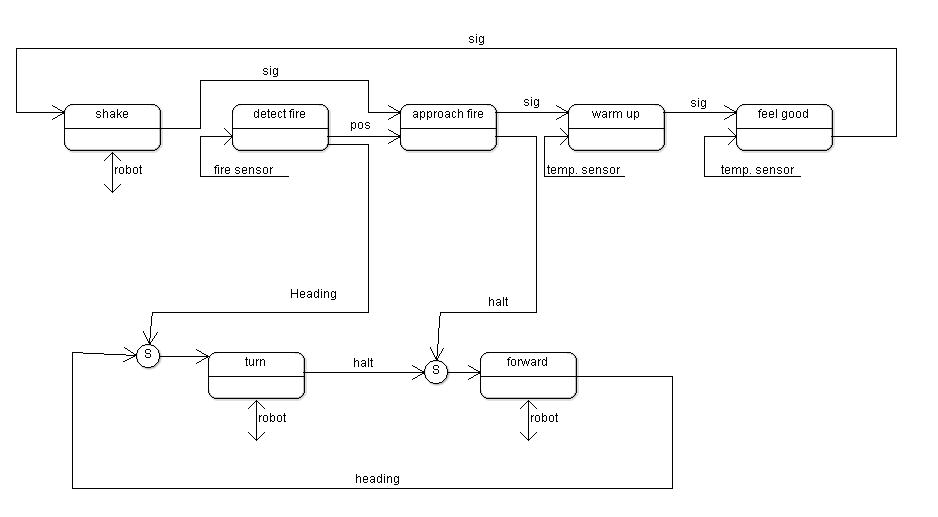
\includegraphics[width=\linewidth]{aufgabe1}
\label{fig:aufgabe1}
\end{figure}

Bei der Erstellung des angegebenen Modells haben wir uns folgendes gedacht:\\
\textbf{Ebene 1:}\\
\begin{itemize}
	\item \texttt{forward} sendet durchgehend eine konstante Richtung nämlich geradeaus. Ansonsten fährt es mit einer konstanten Geschwindigkeit geradeaus solange es kein halt Signal bekommt.
	\item \texttt{turn} bekommt Informationen über die gewünschte Bewegungsrichtung und von einem Hindernissensor beliebiger Art. Mit diesen Informationen dreht \texttt{turn} den Roboter in die richtige Richtung. Es kann den Roboter ebenfalls zum stoppen bringen indem es ein halt Signal an \texttt{forward schickt.}
\end{itemize}\\
\\
\textbf{Ebene 2:}
\begin{itemize}
	\item \texttt{shake} sendet das Schüttelsignal direkt an die Aktuatoren. Weiterhin wird ein start Signal an \texttt{approach fire} gesendet.
	\item \texttt{detect fire} entdeckt mit Hilfe eines geeigneten Sensors ein Feuer und gibt dessen relative Position an \texttt{approach fire} weiter. Dies tut es durchgehend.
	\item \texttt{approach fire} erhält von \texttt{detect fire} durchgehend die relative Position des nächsten Feuers. Sobald ein Startsignal von \texttt{shake} eingegangen ist überschreibt es den heading Eingang von \texttt{turn} um den Roboter in die nähe des Feuers zu bringen. Sobald er in der Nähe ist wird ein Signal an \texttt{warm up} weitergegeben und das Modul schaltet sich ab, bis zum nächsten Startsignal.
	\item \texttt{warm up} erhält Temperaturdaten von einem geeigneten Sensor und schickt so lange ein halt Signal an \texttt{forward} bis der Roboter wieder genügend aufgewärmt ist. Dann sendet es ein Startsignal an \texttt{feel good} und schaltet sich ab.
	\item \texttt{feel good} erhält durchgehend Temperaturdaten von einem geeigneten Sensor und sendet ein Startsignal an \texttt{shake} sobald die Temperatur zu gering ist.
\end{itemize}


\section*{Aufgabe 2}
\subsection*{a)}
\subsection*{b)}
\subsection*{c)}
Wahrscheinlich wollen sie darauf hinaus, dass sich der Rotationspunkt dann besser verhält. Ist aber bei uns abgefangen.

\end{document}
